
\subsection{GDELT Dataset}

\subsubsection{Sparsity in GDELT}

The space of news events spanned by all columns in GDELT is much larger than the subspace we expect news to lie on. Confirming these suspicions is important because it would indicate a need to reduce the dimensionality of the data set we are working with.

Classical dimensionality reduction was not tractable to apply to a dataset of this size - the highly categorical nature of the dataset results in a large dimensional expansion when preparing numeric inputs to the algorithms. A fast neighborhood-embedding method, tSNE, relies only on a metric between data points. Unfortunately, its runtime and space consumption grows exponentially in the reduced dimension, and extremely small dimensions yielded poor results \yrcite{van2008visualizing}.

However, it is critical to observe some sparsity in the GDELT space to confirm our clustering-based approach.

We guessed that there are likely to be at least two modes of low-dimensional interactions in the data: (1) that actors only interact within small cliques and (2) that each actors to small sets of events. We conducted this initial analysis on a random sample of days before August 2015 to avoid making conclusions that overfit the test data.

\begin{figure}[ht]
\vskip 0.2in
\begin{center}
\centerline{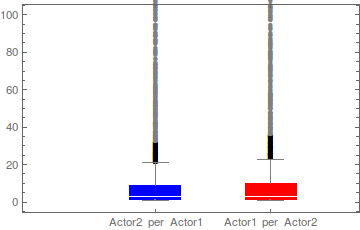
\includegraphics[width=\columnwidth]{images/actors-per-actor.png}}
\caption{Box-and-whisker plot of number of distinct actors each CAMEO actor interacts with (each event may have up to 2 involved actors, where the first inflicts the action), performed on the day-stratified random sample of the events. The medium number of co-actors for both Actor1 and Actor2 categories is 3, with a Q3 of 9 and 10 and maximum of 988 and 990, respectively. The sample contained about 124K events total. The outliers with many interactions are generic or common names, such as \texttt{PRESIDENT} or \texttt{UNITED STATES}.
}
\end{center}
\vskip -0.2in
\label{fig:actors-per-actor}
\end{figure} 

As Figure \ref{fig:actors-per-actor} demonstrates, actor count is heavily skewed distribution. This gives us confidence in (1) for the sampled days. We conduct a similar inspection for the number of unique CAMEO coded events per actor in Figure \ref{fig:events-per-actor}:

\begin{figure}[ht]
\vskip 0.2in
\begin{center}
\centerline{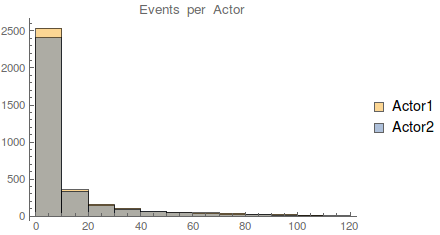
\includegraphics[width=\columnwidth]{images/events-per-actor}}
\caption{Number of events that occur for individual actors. The median actor encounters 3 events, and the 75\% most active ones still see less than 15. This diagram only shows the 95\% least active actors.}
\end{center}
\vskip -0.2in
\label{fig:events-per-actor}
\end{figure} 

In addition to more compact data representation and reduction of noise, dimensionality reduction has several other attractive features for this dataset. First, it enables us to work in a continuous space of reduced-dimension tuples of real values, which is much easier for model generation than partially categorical variables. Secondly, the large volume of the data set implies that any size reductions that can be gained will result in more manageable data pipelines

%\subsection{Bloomberg Commodity Prices}
%up and down spikes
%normally distributed about 0